\documentclass[tikz,border=5pt]{standalone}
\usepackage[UTF8]{ctex}
\usepackage{amsmath}
\usetikzlibrary{arrows.meta,calc}
\definecolor{blue}{RGB}{45,98,142}
\definecolor{green}{RGB}{60,117,87}
\definecolor{red}{RGB}{175,67,51}
\tikzset{vec/.style={thick,-{Stealth}},aux/.style={gray!65,dashed}}
\begin{document}
\begin{tikzpicture}[scale=1.3]
\draw[fill=blue!3](0,0)circle(2.2);
\draw[gray,-{Stealth}](-2.6,0)--(2.8,0)node[right]{$x$};
\draw[gray,-{Stealth}](0,-2.5)--(0,2.6)node[above]{$y$};
\coordinate(A)at(.8,1.38564);\coordinate(B)at(-1.6,0);\coordinate(C)at(.8,-1.38564);
\draw[aux](A)--(B)--(C)--cycle;
\fill(A)circle(1.5pt)node[above right]{$A$};\fill(B)circle(1.5pt)node[above left]{$B$};
\fill(C)circle(1.5pt)node[below right]{$C$};
\fill(0,0)circle(1pt)node[below left]{$O$};
\draw[gray](0,0)--node[midway,left]{$l$}(A);
\coordinate(P)at(.9272,.3746);
\draw[blue,dashed](0,0)--(P)node[midway,above]{$\rho$};
\draw[gray](.45,0)arc(0:22:.45);\node at(.68,.12){$\theta$};
\fill(P)circle(1.2pt)node[above right]{$P$};
\draw[red,vec](P)--++(.3746,-.9272)node[below right]{$F$};
\node at(0,-2.95){俯视：各腿距 $O$ 为 $l$；施力沿顺时针切向};
\end{tikzpicture}
\begin{tikzpicture}[scale=1.3]
\draw[gray!50](0,0)circle(1.6);
\foreach \phi/\name in{60/A,180/B,300/C}{
\coordinate(\name)at(\phi:1.6);
\draw[aux](0,0)--(\name);
\fill(\name)circle(1.3pt)node[shift={(\phi:.22)}]{$\name$};
\draw[blue,vec](\name)--++(0,.65);
\draw[green,vec](\name)--++({-.55*sin(\phi)},{.55*cos(\phi)});
}
\draw[gray](0,0)--(.6,0);\fill(.6,0)circle(1pt)node[above right]{$P$};
\draw[red,vec](.6,0)--(.6,-.6)node[right]{$\boldsymbol F$};
\draw[red,vec](-.35,-.1)arc(196:80:.37);
\node[red]at(-.45,-.4){$-\rho F$};
\node[blue,align=center]at(-2.0,1.7){共同反力\\$-\boldsymbol F/3$};
\node[green,align=center]at(2.1,-1.0){转动反力\\$\dfrac{\rho F}{3l^2}\boldsymbol e_z\times\boldsymbol r_i$};
\node[align=center]at(0,-2.3){$\sum_i\boldsymbol f_i=-\boldsymbol F$\\$\sum_i(\boldsymbol r_i\times\boldsymbol f_i)_z=\rho F$};
\end{tikzpicture}
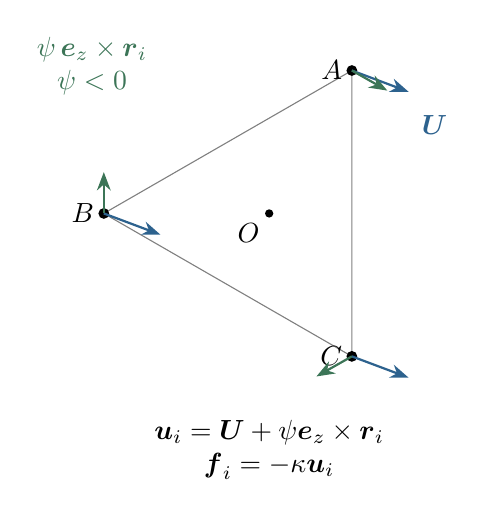
\begin{tikzpicture}[scale=1.5]
\coordinate(A)at(.7,1.21);\coordinate(B)at(-1.4,0);\coordinate(C)at(.7,-1.21);
\draw[gray](A)--(B)--(C)--cycle;\fill(0,0)circle(1pt)node[below left]{$O$};
\foreach \name in{A,B,C}{
\fill(\name)circle(1.3pt)node[left]{$\name$};
\draw[blue,vec](\name)--++(.48,-.18);
}
\draw[green,vec](A)--++(.30,-.17);
\draw[green,vec](B)--++(0,.35);
\draw[green,vec](C)--++(-.30,-.17);
\node[blue]at(1.4,.75){$\boldsymbol U$};
\node[green,align=center]at(-1.5,1.25){$\psi\,\boldsymbol e_z\times\boldsymbol r_i$\\$\psi<0$};
\node[align=center]at(0,-2.0){$\boldsymbol u_i=\boldsymbol U+\psi\boldsymbol e_z\times\boldsymbol r_i$\\$\boldsymbol f_i=-\kappa\boldsymbol u_i$};
\end{tikzpicture}
\begin{tikzpicture}[scale=1.4]
\fill[blue!9](0,0)--(0:2)arc(0:120:2)--cycle;
\fill[green!9](0,0)--(120:2)arc(120:240:2)--cycle;
\fill[red!7](0,0)--(240:2)arc(240:360:2)--cycle;
\draw(0,0)circle(2);
\foreach \phi/\label in{0/0,120/{2\pi/3},240/{4\pi/3}}{
\draw[gray!70](0,0)--(\phi:2);\node at(\phi:2.3){$\theta=\label$};}
\node[blue]at(60:1.2){$A$ 先临界};
\node[green]at(180:1.2){$B$ 先临界};
\node[red]at(300:1.2){$C$ 先临界};
\draw[gray,dashed](0,0)--(60:2);\node[fill=white,inner sep=1pt]at(75:1.7){$R_{\rm t}$};
\fill(0,0)circle(1.1pt)node[below right]{$O$};
\node[align=center]at(0,-2.95){边界上两腿同时临界；圆心三腿同时临界\\条件：三腿相同切向微弹性，固定支持力};
\end{tikzpicture}
\end{document}
